\documentclass[tikz,border=2pt]{standalone}
\usepackage{amsmath}
\usepackage{pgfplots}
\pgfplotsset{compat=1.18}
\usetikzlibrary{arrows.meta}
\begin{document}
% Prisoner's dilemma T=5, R=3, P=1 under grim trigger: cooperating gives R = 3 in every period;
% deviating gives T = 5 once and then P = 1 forever, because the opponent plays D from period 2 on.
% Cooperation is optimal iff 3 >= 5(1-delta) + delta, i.e. delta >= 1/2.
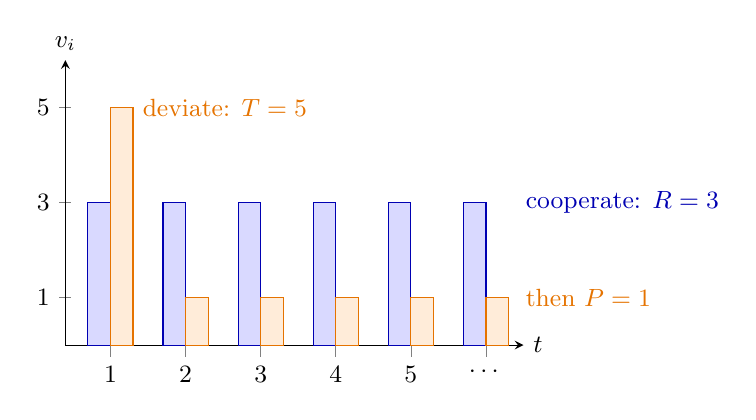
\begin{tikzpicture}[font=\small, >={Latex[length=2mm]}]
  \begin{axis}[
    width=7.4cm, height=5.2cm, axis lines=left,
    xmin=0.4, xmax=6.5, ymin=0, ymax=6,
    xtick={1,2,3,4,5,6}, xticklabels={$1$,$2$,$3$,$4$,$5$,$\cdots$},
    ytick={1,3,5}, xlabel={$t$}, ylabel={$v_i$},
    xlabel style={anchor=west, at={(axis description cs:1,0)}},
    ylabel style={rotate=-90, anchor=south, at={(axis description cs:0,1)}},
    clip=false, every tick label/.append style={font=\small},
    ybar=0pt, bar width=0.3]
    \addplot[draw=blue!70!black, fill=blue!15] coordinates {(1,3) (2,3) (3,3) (4,3) (5,3) (6,3)};
    \addplot[draw=orange!90!black, fill=orange!15] coordinates {(1,5) (2,1) (3,1) (4,1) (5,1) (6,1)};
    \node[orange!90!black, anchor=west] at (axis cs:1.3,5) {deviate: $T=5$};
    \node[blue!70!black, anchor=west] at (axis cs:6.4,3) {cooperate: $R=3$};
    \node[orange!90!black, anchor=west] at (axis cs:6.4,1) {then $P=1$};
  \end{axis}
\end{tikzpicture}
\end{document}
